In this Section, we study the information that we can infer from the dataset about the battles and their evolution throughout history. We start by observing how the duration of the battles and the number of casualties progressed during a millennium. Then, we focus on the outcome of the battles, we try to single out the typical features of a victorious combatant and how we can predict or not the result of a conflict. 

\subsection{Duration of the Battles}

We observe that the duration of the battles over the last millenium increased increased almost continuously. In fact, in Figure \ref{fig:durThByCent}, we observe that the order of magnitude of the duration of a battle has never been higher than nowadays. Notice that the average duration of a battle was almost 34 days during the XX$^{th}$ century while it is currently of 64 days in the XXI$^{st}$ century.

 \begin{figure}[h]
	\centering	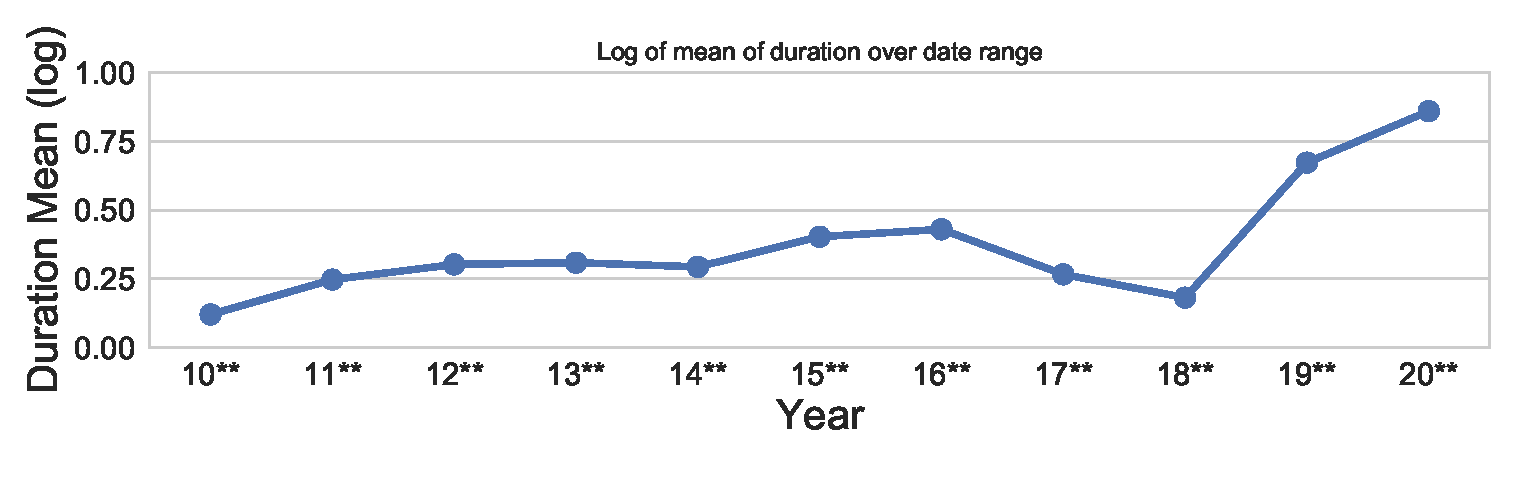
\includegraphics[width=\linewidth]{figures/durThByCent}
	\caption{Mean of the duration of battles in the last thousand years by century on a logarithmic scale.}\label{fig:durThByCent}
	\centering
\end{figure}

\subsection{Evolution of the Casualties}

In Figure \ref{fig:casuPerCent}, we notice that the percentage of soldiers engaged in a battle that are wounded, killed, captured or that disappeared decreases throughout the years. We observe that, following the same trend as shown in Figure \ref{fig:durThByCent} for the battle's duration, the percentage of casualties decreased before increasing in the XX$^{th}$ century. We can infer that in both cases this is due to the world wars because they contain numerous battles which made countless casualties, notably because of technology advances such as aerial forces or gaz attacks.
 \begin{figure}[h]
	\centering	\includegraphics[width=\linewidth]{figures/casuPerCent}
	\caption{Mean of the percentage of casualties in the soldiers.}\label{fig:casuPerCent}
	\centering
\end{figure}

\subsection{Indecisiveness of the Battles}

We observe, in Figure \ref{fig:IndecBattles}, that battles are more indecisive nowadays than they were in the past. In fact, this number (in order of magnitude) is increasing since year 1200 and increased at a higher rate over the last last century. This can be explained by two factors: the first is that battles in the further past were probably often reported by the winner who wouldn't consider it as indecisive. The second is that the two world wars in the  XX$^{th}$ century also contain a lot of strategic and indecisive battles that served a higher or more general goal.
 \begin{figure}[h]
	\centering	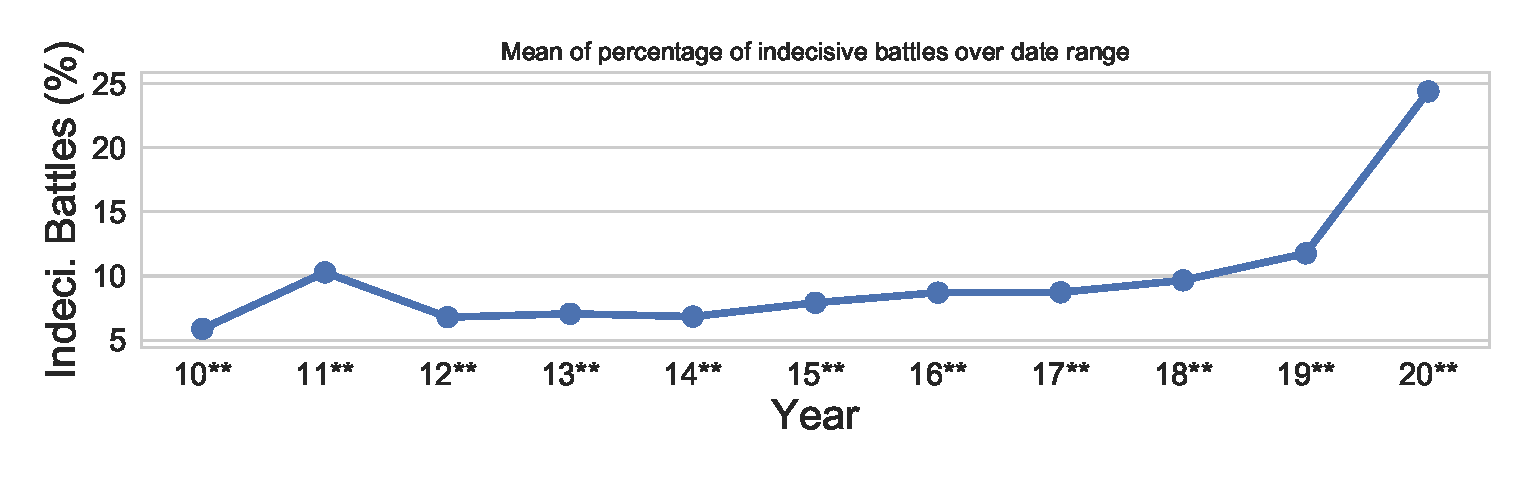
\includegraphics[width=\linewidth]{figures/indThByCent}
	\caption{Mean of the number of indecisive battles over the last thousand years by century on a logarithmic scale.}\label{fig:IndecBattles}
	\centering
\end{figure}

From Figures \ref{fig:durThByCent}, \ref{fig:casuPerCent} and \ref{fig:IndecBattles}, we conclude that battles are longer, make less casualties and are more indecisive over the years. This supports the fact that nowadays the battle's purpose is not only to invade another territory by beating the other combatant. In fact, modern battles seem to be more complicated in the sense that they often serve a higher strategic goal and do not always result in a decisive victory.

\subsection{Outcome of the Battles}

With Figure \ref{fig:victoryAdvantage}, we study the importance for a combatant to have an advantage with respect to the number of casualties (less victims), the number of soldiers (higher strength) and the percentage of casualties among soldiers (casualty ratio). It illustrates the percentage of battles that resulted in a type of victory for a combatant that had an advantage according to one of these features. Our main observation is that the combatant that had less casualties won in almost 80\% of the cases. We noticed that a higher strength resulted in a victory in only less than 50\% of the battles, meaning that in order to predict the winner of a battle, one should simply choose the combatant that suffers less casualties. In order to support our hypothesis, we trained a random forrest classifier on our dataset. Like us, it chose the number of casualties as most important feature to decide the winning side.

We notice that the number of casualties is less important for a strategic victory when the goal is not to inflict more damage to the opponent but to progress towards a more general purpose.
 \begin{figure}[h]
	\centering	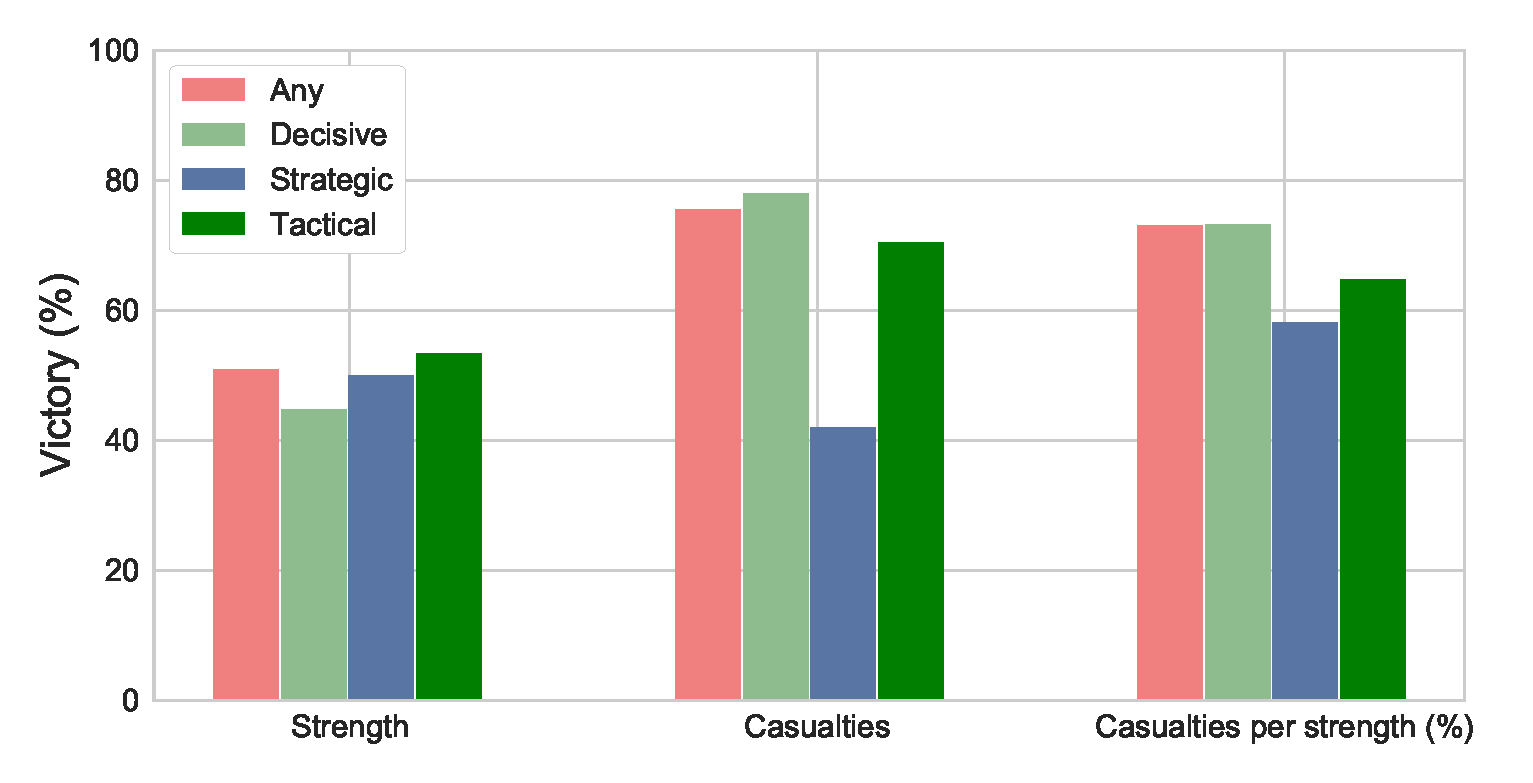
\includegraphics[width=\linewidth]{figures/VictoryAdvantage}
	\caption{Victory percentage with advantage in either strength, casualties or casualty ratio.}\label{fig:victoryAdvantage}
	\centering
\end{figure}

\subsection{Years of Battles per Countries}
In Figure \ref{fig:FightingDurationRanking}, we observe that among all countries in our dataset, France is the one that fought the most. Nevertheless, the United States, which are a major actor in the international history of battles, were only created in 1776 when they proclaimed their independence. Thus, it is interesting to do the same ranking starting from this year. 
 \begin{figure}[h]
 	\centering
 	\begin{subfigure}[b]{0.475\linewidth}
 		\centering
 		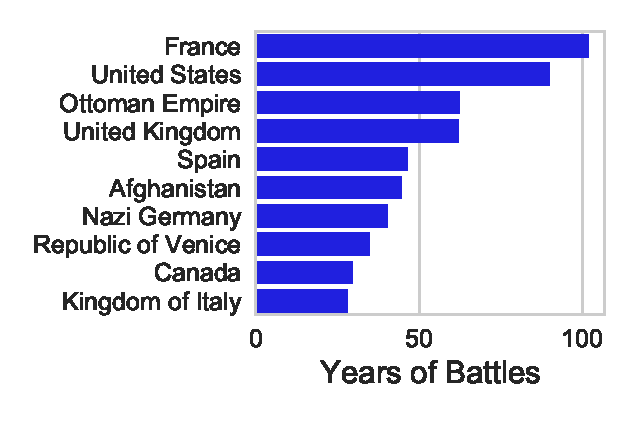
\includegraphics[width=\linewidth]{figures/YearsFightingRanking.eps}
 		\caption[]%
 		{{\small 1000 --- 1700}}    
 		\label{fig:FightingDurationRankingOld}
 	\end{subfigure}
 	\begin{subfigure}[b]{0.475\linewidth}  
 		\centering 
 		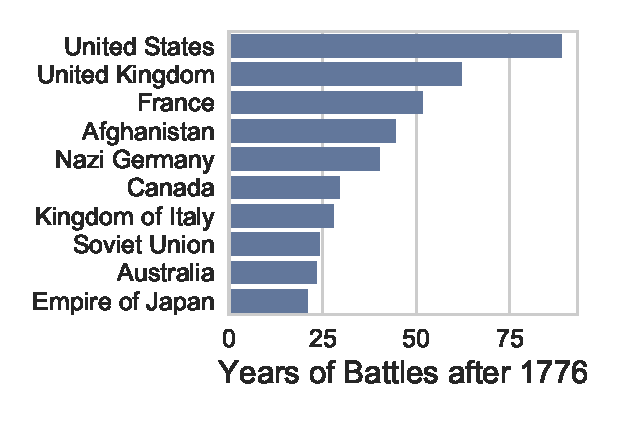
\includegraphics[width=\linewidth]{figures/YearsFightingRankingModern}
 		\caption[]%
 		{{\small 1701 --- 1900}}    
 		\label{fig:FightingDurationRankingModern}
 	\end{subfigure}
 	\vskip0.2\baselineskip
	\caption{Cumulated duration of battles engagement per country. From 100 in (a) and from 1776 and the United States independence in (b).} 
 	\label{fig:FightingDurationRanking}
 \end{figure}
 
 These results tend to support the common belief that the United States are always in war. In fact, as we observe in Figure \ref{fig:USAFightingTimeline}, they were engaged in a at least one battle per year for more than 150 years in 242 years of existence.
 \begin{figure}[h]
 	\centering	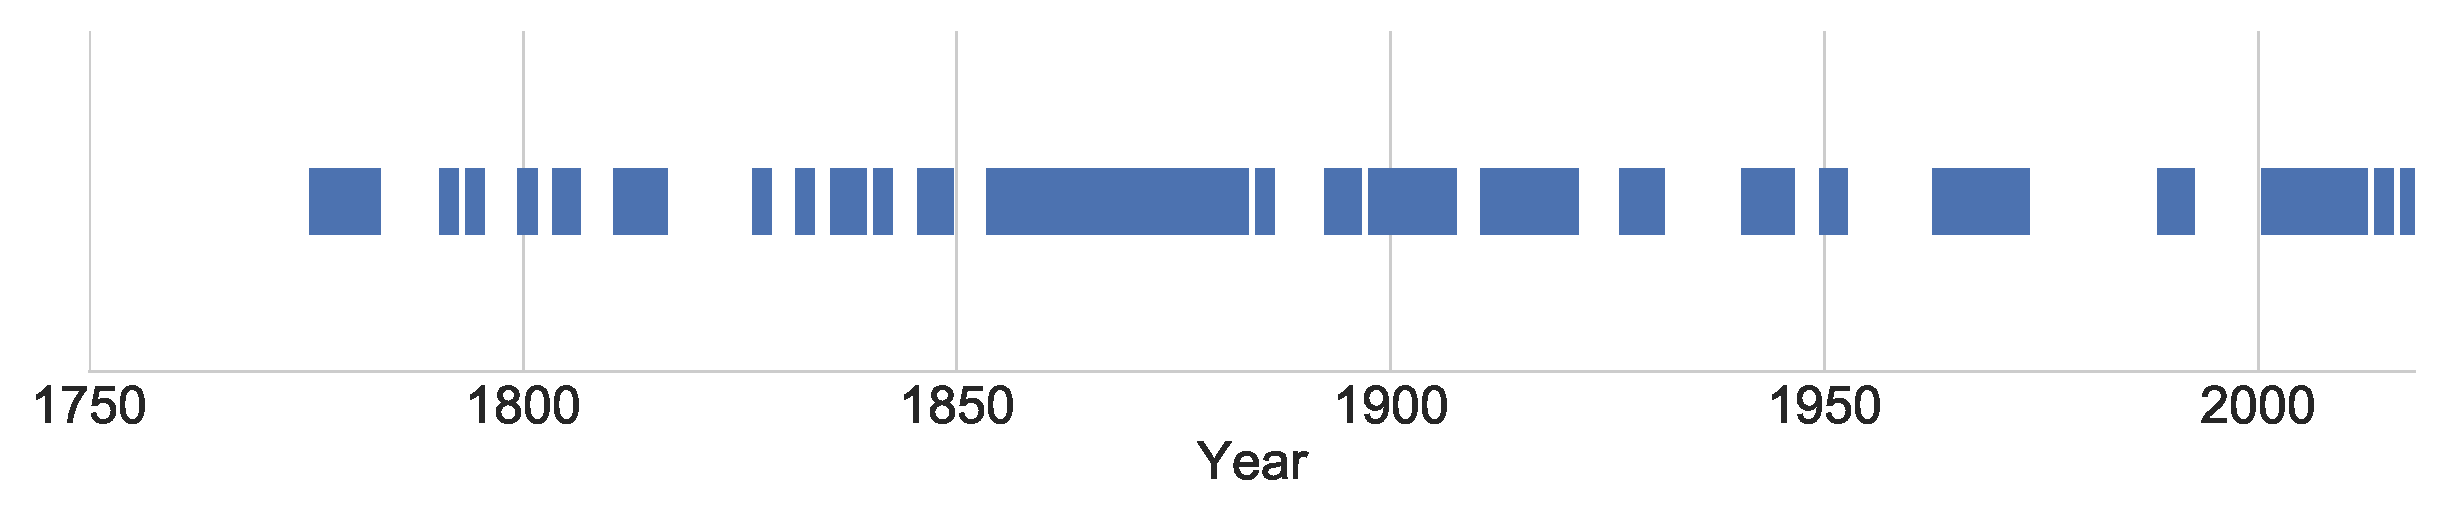
\includegraphics[width=\linewidth]{figures/USAFighting}
 	\caption{Timeline of the USA engagement in battles.}\label{fig:USAFightingTimeline}
 	\centering
 \end{figure}

